\documentclass{article}
\usepackage{CJKutf8}
\usepackage{arxiv}

\usepackage[utf8]{inputenc} % allow utf-8 input
\usepackage[T1]{fontenc}    % use 8-bit T1 fonts
\usepackage{hyperref}       % hyperlinks
\usepackage{url}            % simple URL typesetting
\usepackage{booktabs}       % professional-quality tables
\usepackage{amsfonts}       % blackboard math symbols
\usepackage{nicefrac}       % compact symbols for 1/2, etc.
\usepackage{microtype}      % microtypography
\usepackage{lipsum}
\usepackage{amsthm, amsmath, amssymb, bm}
\usepackage{esvect}
\usepackage{enumerate}
% \newtheorem{theorem}{Theorem}[section]    
\newtheorem{theorem}{Theorem}
\newtheorem{lemma}[theorem]{Lemma}

\usepackage{graphviz}
\usepackage{tikz}
\usetikzlibrary{arrows}
\usetikzlibrary{arrows.meta, calc}
\usetikzlibrary{shapes,positioning,decorations.markings}
\usetikzlibrary{arrows, automata, chains, positioning, shapes.geometric, shapes.symbols}
\usepackage{graphicx}
\usepackage{subcaption}
\usepackage{tikz-qtree}
\usepackage{tikz-qtree-compat}
\usepackage{color}
\usepackage{ upgreek }
\usetikzlibrary{shapes,decorations,arrows,calc,arrows.meta,fit,positioning}
\tikzset{
	-Latex, auto, node distance =1 cm and 1 cm, semithick,
	state/.style ={ellipse, draw, minimum width = 0.7 cm},
	point/.style = {circle, draw, inner sep=0.04cm, fill, node contents={}},
	bidirected/.style={Latex-Latex, dashed},
	el/.style = {inner sep=2pt, align=left, sloped}
}

\theoremstyle{definition}
\newtheorem{definition}{Definition}[section]
 
\theoremstyle{remark}
\newtheorem*{remark}{Remark}
 
\theoremstyle{definition}
\newtheorem{example}{Example}[section]
\newtheorem{principle}[theorem]{Principle}

\newcommand\independent{\protect\mathpalette{\protect\independenT}{\perp}}
\def\independenT#1#2{\mathrel{\rlap{$#1#2$}\mkern2mu{#1#2}}}


% \input{shorts.tex}

\title{{Latex Collector}}


\author{
   Gong Heyang \thanks{Use footnote for providing further
    information about author (webpage, alternative
    address)---\emph{not} for acknowledging funding agencies.} \\
    Univerisity of Science and Technology of China \\
}

\begin{document}
\begin{CJK*}{UTF8}{gbsn}

%%%%%%%%% TITLE
\title{Info Graphical Models}

\author{Gong Heyang\\
University of Science and Technology of China\\
Anhui, Hefei, China\\
{\tt\small zj3712@gmail.com}
% For a paper whose authors are all at the same institution,
% omit the following lines up until the closing ``}''.
% Additional authors and addresses can be added with ``\and'',
% just like the second author.
% To save space, use either the email address or home page, not both
\and
Second Author\\
Institution2\\
First line of institution2 address\\
{\tt\small secondauthor@i2.org}
}

\maketitle
%\thispagestyle{empty}

%%%%%%%%% ABSTRACT
\begin{abstract}
    \emph{Info graph models(IGM)} is a generalization of probabilistic graph models(PGM). 这边文章就是建立一种图模型,边上存储着信息,节点代表量子比特,环代表这序列传播(一种处理原则是直到收敛再传送信息)。 
    \begin{itemize}
        \item 首先回顾各种图模型已经进展到哪里,回答图模型框架的一些基本原则,指出遇到的一些困难。 
        \item 提出我们的建模框架来解决这些困难,我将会看到在我们的建模框架下,本质随机论和量子力学的思想得到了体现,图模型的一些东西的得到了统一。
        \item 从边的理解方面来解释我们的模型,边如何从普通的边推广到我们现在的边。
    \end{itemize}
\end{abstract}

IGM 为了解释生成过程,而PGM更多是为了解释相关性。

\tableofcontents

%%%%%%%%% BODY TEXT
\section{Introduction}

% (模型本质是什么--> 概率模型强调概率 --> 图模型强调表示 --> 我们提出的模型既增强了概率能力,也增强了表示能力。还强调了信息论的观点和生成模型的过程)


模型的本质是什么 ---
A “model,” in the common use of the word, is an idealized representation of reality that highlights some aspects and ignores others\cite{Pearl2009}.
Models are powerful and necessary tools for humans to explore and understand nature and what kinds of modes should we build to achieve human-level machine intelligence has become the central question.

概率模型 ----
Probability models highlights the uncertainty aspects of physical reality. Uncertainty appears to be an inescapable aspect of most real-world applications. It arises because of limitations in our ability to observe the world, limitations in our ability to model it, and possibly even because of innate nondeterminism. Actually, we reveal our objections to Laplace’s (1814) conception of natural phenomena, according to which nature’s laws are deterministic and randomness surfaces owing merely to our ignorance of the underlying boundary conditions. In particularly, all relationships in our models were assumed to be inherently stochastic and thus appeal to the modern (i.e., quantum mechanical) conception of physics, according to which all nature’s laws are inherently probabilistic and determinism is but a convenient approximation.

图模型的作用 ----
The framework of \emph{probabilistic graph models(PGMs)} provides a mechanism for exploiting structure in complex distributions to describe them compactly, and in a way that allows them to be constructed and utilized effectively. PGMs use a graph-based representation as the basis for compactly encoding a complex distribution over a high-dimensional space. There is a dual mathematical perspective that one can use to interpret the structure of graphs: conditional independence and factorization\cite{koller2009probabilistic}

本文提供一个新的通用建模框架 ---
This paper describes a general-purpose framework, which \emph{info graph models(IGMs)}, for constructing and using probabilistic models of complex systems, which can be deemed as a kind of generalization of PGMs. We begin by providing some intuition for the principles underlying this framework, and for the models it encompasses. Complex systems are characterized by the presence of multiple interrelated and generating aspects, many of which relate to the reasoning task. The major focus of IGMs shifts to the generating aspects of complex systems while comparing to PGMs. In the framework of IGMs, we highlight the information perspective of physical reality, thus resulting in significant changes in the interpretations of edges and nodes for a graph leading to a different version of conditional independence criteria and factorization properties.

% The rest of this paper is organized in this way. 
% The IGMs highlight the inherently probabilistic nature of physical process and reality, leading to an new interpretation of nodes and edges in a graph. The PGMs capture relationships more about association over generating aspect which leads to many difficulties on the graph approaches to causal inference. We then highlight the generating aspects of reality by imposing an information processing perspective on graphical models.

\section{Info Graph Models}

概率图模型是大框架,但是与量子理论结合不够 ----
The ideas of PGMs are connected to many fields. From probability theory, we inherit the basic concept of a probability distribution, as well as many of the operations we can use to manipulate it. From computer science, and specifically from artificial intelligence, these models inherit the idea of using a declarative representation of the world to separate procedural reasoning from our domain knowledge. Information theory plays a dual role in providing information-theoretic concepts such as entropy and inference methods based on coding theory. However, the fundamental concepts in quantum theory have not yet turbocharged designing of PGMs, although quantum graphical models have been proposed and also learning and inference algorithms \cite{srinivasan2018learning, leifer2008quantum, jouneghani2013review}. 

We propose our framework of IGMs with the spirit of treating variables(or nodes) in the graph as quantum states. For the binary case of quantum states in quantum computing theory, quantum bits (also called qubits) is in a superposition of both states while a classical bit can be in a '0' or a '1' state. A qubit is both '0' and '1' at the same time until it is “measured.” During measurement or reading, the qubit “collapses” to either a '0' or a '1' with some probability.

% Information theory plays a dual role in its interaction with this field. Information-theoretic concepts such as entropy and information arise naturally in various settings in this framework, such as evaluating the quality of a learned model. On the other side, the recent successes in coding theory, based on the relationship between inference in probabilistic models and the task of decoding messages sent over a noisy channel, have led to a resurgence of work on approximate inference in graphical models.

% Statistics plays an important role both in certain aspects of the representation and in some of the work on learning models from data. Optimization plays a role in providing algorithms both for approximate inference and for learning models from data.

\subsection{Definitions}

We begin by the definition of our proposed framework. Notation $G=(V, E)$ means a graph $G$ with nodes set $V$ and edges set $E$ and $X_S = \{X_v\}_{v\in S}$ for any set $S\subseteq V$.

\begin{definition}[Info Graph Directed Models(IDGMs)]
    An \emph{info directed graph model(IDGM)} by definition consists of:
    \begin{enumerate}[a)]
        \item  A directed graph $G = (V, E)$ associated with a set of variables $X_V$. 
        \item  For every edge $e=(i, j) \in E$, there is a set of samples $S_e$(or $S_{ij}$) which represents the information on $X_i$ that is called the state of edge $e$. 
        \item  For every node $v \in V$, there is an information processing mechanism function $f_v$ which accepts information from its input edges $S_{v^{in}}$ and forces $X_v \sim f_v(S_{v^{in}})$, then sends out by default a sample information $x_v$ to its output edges. 
    \end{enumerate}  
\end{definition}


In an IDGM, nodes or variables  represent the quantum states and the states of edges represent the measured or observed information from the input quantum states. The discussion should not be restricted in the case of directed graphs. Consequently for any graph structure(could be undirected or mixed), we have:

\begin{definition}[Info Graph Models(IGMs)]
    An \emph{info graph model(IGM)} by definition consists of:
    \begin{enumerate}[a)]
        \item  A graph $G = (V, E)$ associated with a set of variables $X_V$. 
        \item  For every edge $e \in E$, there is a set $S_e$ which represents the input information from related variables that is called the state of edge $e$. 
        \item  For every node $v \in V$, there is an information processing mechanism function $f_v$ which accepts information from its input edges $S_{v^{in}}$ , then forcing $X_v \sim f_v(S_{v^{in}})$, and sends out information to its output edges. 
    \end{enumerate}  
\end{definition}

We construct the framework of IGMs inspired by fundamental quantum concepts, thus interpretation of nodes and edges have been very different.

\subsection{Interpretations of Nodes and Edges}

如果某个节点,自己储存状态信息,那么 self-loops 就是这个玩意儿。

边也会选择连接的个体,网络结构的形成应该是一个剪枝的过程。

The first rule of understanding the construction of the framework is the symmetry property of edges and nodes in graphs.

\begin{principle}[Symmetrical View of Nodes and Edges]
\label{prin:sym}
In the framework of IGMs, nodes are affected by information from its input edges, and edges collect information from its input nodes.
\end{principle}

这种对称性类比超图 ---
Actually, this symmetrical treatment is originate from a strict mathematical concept. Contrast to commonly used graphs which define edges between two different nodes, a graph that allows edges connect a set of nodes(called hyperedges, e.g. self-loops) is referred as \emph{hypergraph} with the mathematical symmetrical property of edges and nodes, which have been extensively used in machine learning tasks as the data model and classifier regularization\cite{zhou2007learning}. This principle suggest that information can affect many nodes, and a nodes can be observed or measured by many edges. 

IGMs 框架具备信心论的理解。
The IGMs have strong connections to information theory just as PGMs do. Information theory plays a dual role in its interaction with PGMs. Information-theoretic concepts such as entropy and information arise naturally in various settings in this framework, such as evaluating the quality of a learned model. On the other side, the recent successes in coding theory, based on the relationship between inference in probabilistic models and the task of decoding messages sent over a noisy channel, have led to a resurgence of work on approximate inference in graphical models. Additionally, every nodes in our framework can be deemed as an information processing subsystem, and using edges to keep in track of the nodes observation information. 

The quantum and information perspectives emphasised by the IGMs framework lead to the following principle:

\begin{principle}[Quantum Understanding of Nodes]
\label{prin:quantum}
In the framework of IGMs, every node represent a quantum state which evolves according to its environment information.
\end{principle}

关于state的理解---

All Information are on edges and nodes state associate with a "collapse" distribution according to this principle. Carefully interpretation of the word "state" should be taken. Taking hidden Markov models (HMMs) for example, the hidden state of a sequence in this setting is quite different from the state of a node in our IGMs, which should be interpreted as quantum state. And the state of an edge in IGMs represents the information collected from related nodes. Moreover, the HMMs indicate a situation where state information of a node is useful, which against the idea of our interpretation of nodes as quantum states. In this case, we can add a self-loop(a directed edge with the same start and end nodes) to collect information of a node.

Now let's turn to one of the most important question of graphical model: "How graphs encodes can encode conditional independencies between random variables, or equivalently, a factorization of joint distribution of the variables."

\section{Representation} \label{sec:repre}


% 最重要的是独立性,独立机制的性质。
An idea graphical models framework should allow us to choreograph a parsimonious and modular representation of the domain knowledge of variety given problems, interrogate that representation and finally answer inferential questions correctly with ease. 

\subsection{Graphs with Cycles}

In the framework of PGMs, directed graphs are useful for representing conditional independence relations among variables. % They are also used to represent causal relationships. 
But we encounter both interpretation and computation difficulties when it comes to the case of cyclic directed graphs while cycles are usually used to represent feedbacks of a given problem\cite{bongers2016theoretical}. For example, 

\begin{example}[Cyclic Directed Graph Model]
\label{eg:cycleDG}
For an graphical model $G=(V, E)$ with nodes $A, B, C \in V$ and three directed edges $\vv{AB}, \vv{BC}, \vv{CA} \in E$ which forms a cycle, the conditional independencies between variables, or equivalently the associated factorization property, can not be easily introduced.   


\begin{figure}[h]
	\begin{subfigure}[tb]{0.45\textwidth}
		\centering
		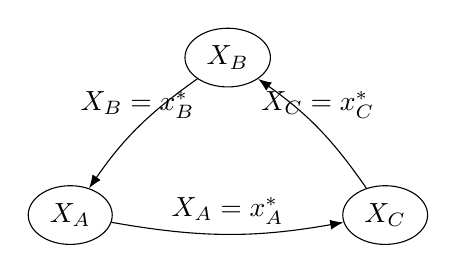
\begin{tikzpicture}
		\node[state] (x) at (0, 0) {$X_A$};
		\node[state] (z) at (2, 2) {$X_B$};
		\node[state] (y) at (4, 0) {$X_C$};
		
		% Directed edge
		\path (x) edge[bend right=10, align=right, above] node {$X_A=x_A^*$} (y);
		\path (y) edge[bend right=10, align=left, above] node {$X_C=x_C^*$} (z);
		\path (z) edge[bend right=10, align=left, above] node {$X_B=x_B^*$} (x);
		\end{tikzpicture}
		\caption{Case 1: Information on edges are just a sample of its input nodes.}
		\label{fig:onesample}
	\end{subfigure}
    \hfill
	\begin{subfigure}[tb]{0.45\textwidth}
		\centering
		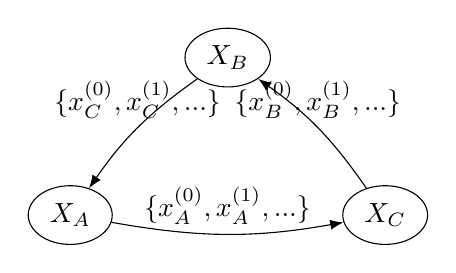
\begin{tikzpicture}
		\node[state] (x) at (0, 0) {$X_A$};
		\node[state] (z) at (2, 2) {$X_B$};
		\node[state] (y) at (4,0) {$X_C$};
		
		% Directed edge
		\path (x) edge[bend right=10, align=right, above] node {$\{x_A^{(0)}, x_A^{(1)}, ...\}$} (y);
		\path (y) edge[bend right=10, align=left, above] node {$\{x_B^{(0)}, x_B^{(1)}, ...\}$} (z);
		\path (z) edge[bend right=10, align=left, above] node {$\{x_C^{(0)}, x_C^{(1)}, ...\}$} (x);
		\end{tikzpicture}
		\caption{Case 2: Information on edges are a sequence of samples of its input nodes.}
		\label{fig:manysamples}
	\end{subfigure}\caption{Information on edges.}
\end{figure}

\end{example}

Markov性质 ----
We will show that, in our framework of IGMs, many directed graphs with cycles such as this simple cyclic graph with three nodes would have a natural interpretation. Markov properties for PGMs which may be characterized by factorized densities relate to local properties of the model and the counterpart in our framework can be stated by the following principle:

\begin{principle}[Independent Mechanisms]
    For any two disjoint sets of variables $X, Y$ in the an IGM, $X$ and $Y$ are conditionally independent given there corresponding information from their input edges.
\end{principle}

In an IGM on the graph in Example \ref{eg:cycleDG}, the nodes denoted as $X_A, X_B, X_C$ associated with densities $f_A, f_B, f_C$ satisfy that 

\begin{equation} \label{eq:1}
\left\{
     \begin{array}{lr}
     X_A \sim f_A(x_A|s_{CA}) &  \\
     X_B \sim f_B(x_B|s_{AB}) & \\
     X_C \sim f_C(x_C|s_{BC}) &  
     \end{array}
\right.
\end{equation}

where $s_{AB}, s_{BC}, s_{CA}$ are information on corresponding edges.

For the simplest case in Figure \ref{fig:onesample} of Example \ref{eg:cycleDG}, let's say, if the information on edge $\vv{AB}$ is an event $X_B=x_B^*$, and similarly for $s_{BC}, s_{CA}$, then we could have:

\begin{equation}
\left\{
     \begin{array}{lr}
     X_A \sim f_A(x_A|x_{C}^*) &  \\
     X_B \sim f_B(x_B|x_{A}^*) & \\
     X_C \sim f_C(x_C|x_{B}^*) &  
     \end{array}
\right.
\end{equation}

In other words, edges collect observations $(x_A, x_B, x_C)$ of nodes and nodes are affected by information $(x_A^*, x_B^*, x_C^*)$ on its input edges. 

For a more general case in Figure \ref{fig:manysamples} of Example \ref{eg:cycleDG}, if the information on corresponding edges are a sequence of observations of its input nodes, then we can propose an underlying information processing procedure according the Principle \ref{prin:sym} where edges and nodes are updated alternately at each step $t$ by

\begin{equation} \label{eq:evolve}
\left\{
     \begin{array}{lr}
     X_A^{(t+1)} \sim f_A(x_A|s_{C}^{(t)}) &  \\
     X_B^{(t+1)} \sim f_B(x_B|s_{A}^{(t)}) & \\
     X_C^{(t+1)} \sim f_C(x_C|s_{B}^{(t)}) &  
     \end{array}
\right.
\end{equation}

and 

\begin{equation} \label{eq:collect}
\left\{
     \begin{array}{lr}
     s^{(t+1)}_C = s^{(t)}_C \cup \{x_C^{(t+1)}\}, & x_C^{(t+1)} \sim X_C^{(t+1)} \\
     s^{(t+1)}_B = s^{(t)}_B \cup \{x_B^{(t+1)}\}, & x_B^{(t+1)} \sim X_B^{(t+1)} \\
     s^{(t+1)}_A = s^{(t)}_A \cup \{x_A^{(t+1)}\}, & x_A^{(t+1)} \sim X_A^{(t+1)}  
     \end{array}
\right.
\end{equation}

where $s_{C}^{(t)} = \{x^{(t)}_C, ..., x^{(0)}_C\}$ and $x_C^{(t+1)} \sim X_C^{(t+1)}$ means $x_C^{(t+1)}$ is a sample of $X_C^{(t+1)}$. 

Updating Equations \ref{eq:evolve} reflect the Principle \ref{prin:quantum}, which indicates that the nodes in the graph recursively affect by information from its input edges $s^{(t)}$. Of course, updating rules defined by Equations \ref{eq:evolve} and Equations \ref{eq:collect} can be specified according to the specific domain problems which is why IGMs are considered as a general framework of modeling physical reality. 

\subsection{PID Control Systems}

另外一个可以使用我们图框架进行描述的在工业界被广泛使用的模型是 PID 控制系统( PID controller)。PID控制系统是这样..(A PID controller is an instrument used in industrial control applications to regulate temperature, flow, pressure, speed and other process variables. PID (proportional integral derivative) controllers use a control loop feedback mechanism to control process variables and are the most accurate and stable controller.)
在我们的框架下,他可以这样理解:


\begin{figure}[h]
	\begin{subfigure}[tb]{0.45\textwidth}
		\centering
        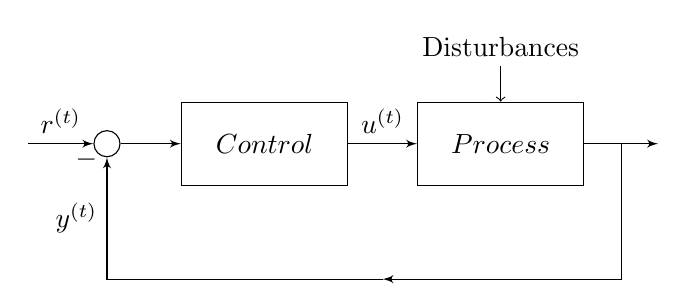
\begin{tikzpicture}[auto, node distance=2cm,>=latex']
            \tikzstyle{block} = [draw, fill=white, rectangle, 
                minimum height=3em, minimum width=6em]
            \tikzstyle{sum} = [draw, fill=white, circle, node distance=1cm]
            \tikzstyle{input} = [coordinate]
            \tikzstyle{output} = [coordinate]
            \tikzstyle{pinstyle} = [pin edge={to-,thin,black}]
            \node [input, name=input] {};
            \node [sum, right of=input] (sum) {};
            \node [block, right of=sum] (controller) {$Control$};
            \node [block, right of=controller,
            pin={[pinstyle]above:Disturbances},
                    node distance=3cm] (system) {$Process$};
        
            \draw [->] (controller) -- node[name=u] {$u^{(t)}$} (system);
            \node [output, right of=system] (output) {};
            \node [input, below of=u] (measurements) {Measurements};
        
            \draw [draw,->] (input) -- node {$r^{(t)}$} (sum);
            \draw [->] (sum) -- node {} (controller);
            \draw [->] (system) -- node [name=y] {}(output);
            \draw [->] (y) |- (measurements);
            \draw [->] (measurements) -| node[pos=0.99] {$-$} 
                node [near end] {$y^{(t)}$} (sum);
 
        \end{tikzpicture}
		\caption{A typical PID control system.}
		\label{fig:pid1}
	\end{subfigure}
    \hfill
	\begin{subfigure}[tb]{0.45\textwidth}
		\centering
    	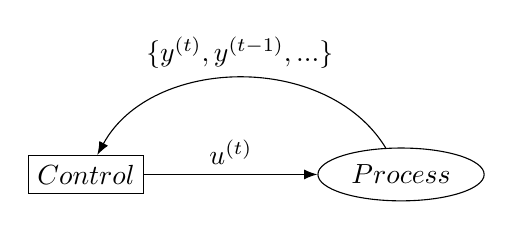
\begin{tikzpicture}
    	\node[state, shape=rectangle] (x) at (0, 0) {$Control$};
    % 	\node[state, shape=rectangle] (z) at (-2, 0) {$r(t)$};
    	\node[state] (y) at (4, 0) {$Process$};
    	
    	% Directed edge
    	\path (x) edge[bend right=0, align=right, above] node {$u^{(t)}$} (y);
    	\path (y) edge[bend right=60, align=left, above] node {$\{y^{(t)}, y^{(t-1)}, ... \}$} (x);
    % 	\path (z) edge (x);
    	\end{tikzpicture}
		\caption{IGM view of typical PID control system}
		\label{fig:pid2}
	\end{subfigure}\caption{Information on edges.}
\end{figure}

在这种情况下 Fig \ref{fig:pid1} 中我们的更新公式是
 $$
 u^{(t)}=K_{\text{p}} e^{(t)}+K_{\text{i}}\sum_{t'\leq t}e^{(t')}\, +K_{\text{d}} \Delta e^{(t)},
 $$

where $K_{\text{p}}, K_{\text{i}}$, and $K_{\text{d}}$, all non-negative, denote the coefficients for the proportional, integral, and derivative terms respectively (sometimes denoted $P$, $I$, and $D$).

对应的,在 Fig \ref{fig:pid1} 中我们的更新公式是


\begin{equation} \label{eq:evolve}
\left\{
     \begin{array}{lr}
     Y^{(t+1)} \sim f_Y(y|s_{\vec{UY}}^{(t)}) &  \\
     U^{(t+1)} \sim f_U(u|s_{\vec{YU}}^{(t)}) & \\
     \end{array}
\right.
\end{equation}

and 

\begin{equation} \label{eq:collect}
\left\{
     \begin{array}{lr}
     s^{(t+1)}_{\vec{UY}} = \{u^{(t+1)}\}, & u^{(t+1)} \sim U^{(t+1)} \\
     s^{(t+1)}_{\vec{YU}} = s^{(t)}_A \cup \{y_{(t+1)}\}, & y^{(t+1)} \sim Y^{(t+1)}  
     \end{array}
\right.
\end{equation}

这是带环的一个典型的系统,体现了我们框架的强大的表达能力。

带环的概率图模型是最难处理,我们提供了一种表示和处理的信息框架。同样对于现在广泛应用的DAGs,我们也有一些洞见。

\subsection{Stochastic Computation Graphs}

从概率变成到随机计算图 ---
In the recent years, Probabilistic programming (PP) is a programming paradigm in which probabilistic models are specified and inference for these models is performed automatically. It represents an attempt to unify probabilistic modeling and traditional general purpose programming in order to make the former easier and more widely applicable. Many probabilistic programming languages have been developed for PP, such as Pyro, Gen, Edward, which are based on a key mathematical concepts --- statistic computation graphs (SCGs). SCGs are directed acyclic graphs that include both deterministic functions and conditional probability distributions which could assist researchers in developing intricate models involving a combination of stochastic and deterministic operations, enabling, for example, attention, memory, and control actions.  

\begin{definition}[Stochastic Computation Graphs(SCG)]
A directed, acyclic graph, with three types of nodes:
\begin{enumerate}[(1)]
    \setlength\itemsep{-0.5em}
    \item Input nodes, which are set externally, including the parameters we differentiate with respect to.
    \item Deterministic nodes, which are functions of their parents.
    \item Stochastic nodes, which are distributed conditionally on their parents.
\end{enumerate}

Each parent $v$ of a non-input node $w$ is connected to it by a directed edge $(v, w)$.
\end{definition}

我们一般使用 circles 代表随机节点, rectangles for 确定性节点。---
The SCGs generalize directed graphical models where stochastic nodes are denoted with circles and Deterministic nodes are denoted with rectangles.





What we have learn from the recently dramatic success in machine learning in the past three decades is that representation first. Learning the features of a given problem has become a more important task than prediction. You can peep from this simple example that our framework many have a stronger representation power for complex systems with feedbacks though details of this view go beyond this paper. Bayesian networks are one kind of most widely used probabilistic graph models in many areas, which can be treated as a special case of IDGMs. Actually, the the Temporal property of dynamic Bayesian networks can be induced by updating rules like Equations ref{eq:evolve} and Equations \ref{eq:collect} given some appropriate settings of the edges information collecting and the nodes state evolving.

% 我们尝试使用这个例子来说我们框架的优越性,当然很多研究者并不会轻易相信。包括我在内都会提出质疑。那么我们先从最简单的例子出发来说明至少不是不差于PGMs 框架就很有必要。小面我们从贝叶斯网络出发,说明它是我们的一种特殊情况。
Although PGMs are a general-purpose framework for constructing and using probabilistic models of complex systems and they have made a significant impact on a broad spectrum of real-world applications in different areas, we argue that new interpretations of nodes and edges should be taken for graphical models in probabilistic view of reality, thus we propose a new framework of IGMs. Indeed, agent-based models will be a good example that reveal the representation power of our framework for modeling complex systems.

% 图模型已经取得的很多成就,具备强大的表达能力,为什么还需要我们的推广呢?


\section{IGMs for Complex Systems}

提出新新的原则,任何子模型都是一个信息处理机制,是一个计算模型。


(复杂系统)Complex systems are characterized by the presence of multiple interrelated aspects, many of which relate to the reasoning task. 
% For example, in our medical diagnosis application, there are multiple possible diseases that the patient might have, dozens or hundreds of symptoms and diagnostic tests, personal characteristics that often form predisposing factors for disease, and many more matters to consider. 
IGMs have shown their advantage on overcome theoretical impediments on systems with cycles, and we now also show example how it facilitate modeling of complex empirical science problems.

\subsection{Agent-based Models in Economic}

ABM是什么?---
An agent-based model (ABM), to some extent evolved from Cellular Automata (CA), is a class of computational models for simulating the actions and interactions of autonomous agents with a view to assessing their effects on the system as a whole, which is widely used in many empirical science such as social science, economics. Leigh Tesfatsion summarize five essential properties in real-world economies, 

\begin{itemize}
    \item  First, they consist of heterogeneous interacting participants characterized by distinct local states (data, attributes, methods) at each given time. 
    \item Second, they are open-ended dynamic systems whose dynamics are driven by the successive interactions of their participants. 
    \item Third, human participants are strategic decision-makers whose decision processes take into account past actions and potential future actions of other participants. 
    \item Fourth, all participants are locally constructive, i.e., constrained to act on the basis of their own local states at each given time. 
    \item Fifth, the actions taken by participants at any given time affect future local states and hence induce system reflexivity.
\end{itemize}

These five essential properties imply that real-world economies are hard to model with PGMs and lead to agent-based computational economics (ACE)\cite{tesfatsion2006handbook, tesfatsion2002agent}, in contrast, they can be characterized by IGMs if we treat agents as node and edges as channels through which agents interacting. In particularly, they can be naturally interpreted in IGMs framework:

\begin{itemize}
    \item First, nodes interacting by sending and accepting information on edges(self-loops represent states of nodes)
    \item Second, nodes evolve according to edges information and edges collect information from nodes intrinsically imply a dynamic process.
    \item Third, nodes evolve according to mechanism functions $f_v$ which take collected edges states (which could include both present and past information) as inputs.
    \item Fourth, nodes are independently affected by information from its inputs information locally.
    \item Reflexivity refers to circular or feedback loops which has been discussed in previous Section \ref{sec:repre}.
\end{itemize} 


IGMs是会在全方位帮助发展 ACE 理论。---
The framework of IGMs will help serve as a tool for ACE research on empirical understanding, normative design, qualitative insight and theory generation, and method/tool advancement. 






\subsection{Marginalizing and Sub-models}

边也会选择连接的个体,网络结构的形成应该是一个剪枝的过程。边是信息实体,例如一本书,选择了某些个体连接起来。


====> 和 ABM 联系,关于信息处理,类比人类社会的沟通 with voice。他们能被听懂是因为人脑能处理声音信号。声音信号能够大大的一群人的行为是一个非常美妙的事情,几乎就是一点单的能量,完成了无数的事情。因果计算链条一旦开启,那么高熵的智能系统能够完成不可思议的计算。人类制造如此精密大飞机,靠的是整个人类社会的密切合作,没有一个人能够单独制造出大飞机,但是人类之间多层级复杂连接结构让群体智能成为可能。


====> 图模型使用的最大问题是不知道网络结构,网络结构并不是人类设计出来的,理想的网络结构应该是群体演化出来。物种内的道德机制和竞争机制相互制衡。个体之间的相互协作和竞争都需要存在,所以网络节点的增加或者删除是通过演化决定的。一个实际问题的网络结构,如何从无到有演化出来呢?需要两个问题,如何增加网络宽度和深度的规则设计。深度可以通过剪枝完成,宽度可以通过复制完成 based on DenseNet。




\subsection{智能网络观点}

有些问题是不可约化的复杂,解决复杂的问题需要复杂的工具,使用复杂对抗复杂。计算底层物理系统的复杂性也非常重要。

一个有生命的系统和非生命的系统是不同的。前者是一个开放的系统,需要和外界进行物质、能量或者信息的交换。后者为了其稳定性,需要和外界隔绝,才能保持其独立性,比如一瓶纯净的氧气,盖子一旦打开,就和周围环境中的空气相混合,就不再是纯氧了。

\section{Causality}

indeterminism


因果一定存在能量交换,一定会发送信息,信息的传输是不能超过光速的。


Pearl's recently propose the \emph{mini-Turning test} that  How can machines represent causal knowledge in a way that would enable them to access the necessary information swiftly, answer questions correctly, and do it with ease, as a human can? 

因果是强AI的组建,更加关注的是推断过程,在微观层次上决策是先于解释的,解释就是因果理论的主要功能。


因果并不存在,但是是一种非常有用的幻觉。在我们的框架中, 量子态之间并不存在直接相互影响,事件之间有因果关系吗?也没有。

因果的定义

{Philosophy and Principles}

Reichenbach's principle asserts that if two observed variables are found to be correlated, then there should be a causal explanation of these correlations. 



\subsection{waited}

Although the framework we describe here shares common elements with a broad range of other topics, it has a coherent common core: the use of structure to allow a compact representation, effective reasoning, and feasible learning of general-purpose, factored, probabilistic models. These elements provide us with a general infrastructure for reasoning and learning about complex domains.


As we discussed earlier, by using a declarative representation, we essentially separate out the description of the model for the particular application, and the general-purpose algorithms used for inference and learning. Thus, this framework provides a general algorithmic toolkit that can be applied to many di erent domains.

Indeed, probabilistic graphical models have made a significant impact on a broad spectrum of real-world applications. For example, these models have been used for medical and fault diagnosis, for modeling human genetic inheritance of disease, for segmenting and denoising images, for decoding messages sent over a noisy channel, for revealing genetic regulatory pro- cesses, for robot localization and mapping, and more. Throughout this book, we will describe how probabilistic graphical models were used to address these applications and what issues arise in the application of these models in practice.

In addition to practical applications, these models provide a formal framework for a variety of fundamental problems. For example, the notion of conditional independence and its explicit graph-based representation provide a clear formal semantics for irrelevance of information. This framework also provides a general methodology for handling data fusion — we can introduce sensor variables that are noisy versions of the true measured quantity, and use Bayesian conditioning to combine the different measurements. The use of a probabilistic model allows us to provide a formal measure for model quality, in terms of a numerical fit of the model to observed data; this measure underlies much of our work on learning models from data. The temporal models we define provide a formal framework for defining a general trend toward persistence of state over time, in a way that does not raise inconsistencies when change does occur.

In general, part of the rich development in this field is due to the close and continuous interaction between theory and practice. In this field, unlike many others, the distance between theory and practice is quite small, and there is a constant flow of ideas and problems between them. Problems or ideas arise in practical applications and are analyzed and subsequently developed in more theoretical papers. Algorithms for which no theoretical analysis exists are tried out in practice, and the profile of where they succeed and fail often provides the basis for subsequent analysis. This rich synergy leads to a continuous and vibrant development, and it is a key factor in the success of this area.





\section{Conclusion}

In summary, the IGMs highlight the inherently probabilistic nature of physical process and reality, leading to an new interpretation of nodes and edges in a graph. The PGMs capture relationships more about association over generating aspect which leads to many difficulties on the graph approaches to causal inference. We then highlight the generating aspects of reality by imposing an information processing perspective on graphical models.

%(表示复杂系统的时候遇到一些限制)

The traditional framework of probabilistic graph models address many of the limitations present in representation of complex systems. Though we think we have identified some weaknesses in the interpretations of edges and nodes in graphs, we do not wish to suggest that this somehow taints the tools and methods that many graph models have advocated, extended or developed in the framework of PGMs. We are in strong agreement with that PGMs are a very valuable framework for modeling physical reality and performing inference with it. If anything our criticism of the traditional PGMs is that it is not ‘probabilistic enough’ in the sense that, as we have seen, since the uncertainty nature of physical reality in the quantum level presents as a ground truth. In contrast, our framework of IGMs, rooted in the non-determinism philosophy or belief, puts emphasis on the information passing perspective of complex computing systems. And we have shown many kinds of PGMs can be seem as a special kinds of IGMs.




{\small
\bibliographystyle{ieee_fullname}
\bibliography{egbib}
}

\end{CJK*}
\end{document}
